% questions.tex —— 1999 年·上海卷·文史类 · 题目内容片段（无答案）
% 由 tools/generate_projects.py 依来源总账自 1999/1999_数学真题_上海文_试题.md 生成，勿手改（改源 MD 后重跑）


\begin{gktip}
来源说明：本稿已按固定扫描件完成22题题面逐页转录与主审复核；卷内答案已独立转录，并与盲解和题面逐题对照。Q13、Q19题面与卷内答案冲突，Q21（2）疑有源文问题仍待核；Q8、Q20、Q21图稿按扫描页重绘并完成四版校样。扫描件无文字层，按渲染页图核读，未使用 OCR。卷首写明全卷 22 题、满分 150 分：填空 1–12（每题 4 分），选择 13–16（每题 4 分），解答 17–22（共 86 分）。卷内含答案要点及评分标准；只在来源转录中称“卷内所载”，不代表官方答案。来源固定字节与卷首自题不证明出版者或版次。

源文待核：第 16 题末项标签在扫描页中与首项相同，均印作“A”；第 21 题（2）“如图所示形状的几何体积为柱体”语句疑似有排印缺字，暂照录。第 8、20、21 题的矢量图按固定扫描页重绘并分别链接；图中只表达原图标注与示意关系，不表示比例。
\end{gktip}

\gkpart{一、填空题（1—12，每题 4 分，共 48 分）}

本大题共有 12 题，只要求直接填写结果；每个空格填对得 4 分，否则一律得零分。

\begin{question}
\gkti{1}$\operatorname{tg}\left[\arccos\frac{\sqrt2}{2}-\frac\pi6\right]=$ \gkblank{}。

\end{question}
\begin{question}
\gkti{2}函数 $f(x)=\log_2 x+1\ (x\ge4)$ 的反函数 $f^{-1}(x)$ 的定义域是 \gkblank{}。

\end{question}
\begin{question}
\gkti{3}在 $\left(x^3+\frac{2}{x^2}\right)^5$ 的展开式中，含 $x^5$ 项的系数为 \gkblank{}。

\end{question}
\begin{question}
\gkti{4}在 $\triangle ABC$ 中，若 $\angle B=30^\circ$，$AB=2\sqrt3$，$AC=2$，则 $\triangle ABC$ 的面积 $S$ 是 \gkblank{}。

\end{question}
\begin{question}
\gkti{5}若平移坐标系，将曲线方程 $y^2+4x-4y-4=0$ 化为标准方程，则坐标原点应移到点 $O'(\underline{\qquad},\underline{\qquad})$。

\end{question}
\begin{question}
\gkti{6}函数 $y=2\sin x\cos x-2\sin^2x+1$ 的最小正周期 $T=$ \gkblank{}。

\end{question}
\begin{question}
\gkti{7}函数 $y=2\sin\left(2x+\frac\pi6\right)\ (x\in[-\pi,0])$ 的单调递减区间是 \gkblank{}。

\Needspace{0.4\textheight}
\end{question}
\begin{question}
\gkti{8}某工程的工序流程图如下（工时单位：天）。
\nopagebreak[4]
\begin{center}% 1999 上海文科 Q8：按固定扫描页重绘；实线为工序，虚线为零工时虚活动。
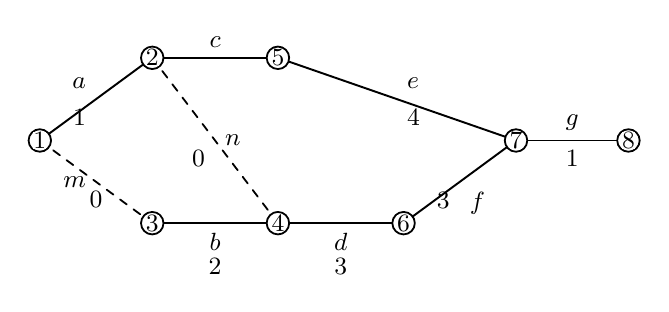
\begin{tikzpicture}[>=stealth, line join=round, line cap=round, scale=0.84,
  every node/.style={font=\small}]
  \tikzset{activity/.style={->, line width=0.7pt}, dummy/.style={->, dashed, line width=0.65pt}}
  \coordinate (n1) at (0,0);
  \coordinate (n2) at (1.7,1.25);
  \coordinate (n3) at (1.7,-1.25);
  \coordinate (n4) at (3.6,-1.25);
  \coordinate (n5) at (3.6,1.25);
  \coordinate (n6) at (5.5,-1.25);
  \coordinate (n7) at (7.2,0);
  \coordinate (n8) at (8.9,0);

  \draw[activity] (n1)--node[above left] {$a$} node[below left] {$1$} (n2);
  \draw[dummy] (n1)--node[left] {$m$} node[below] {$0$} (n3);
  \draw[activity] (n3)--node[below] {$b$} node[below=9pt] {$2$} (n4);
  \draw[dummy] (n2)--node[right] {$n$} node[below left] {$0$} (n4);
  \draw[activity] (n2)--node[above] {$c$} (n5);
  \draw[activity] (n4)--node[below] {$d$} node[below=9pt] {$3$} (n6);
  \draw[activity] (n5)--node[above right] {$e$} node[below right] {$4$} (n7);
  \draw[activity] (n6)--node[below right] {$f$} node[below left] {$3$} (n7);
  \draw[activity] (n7)--node[above] {$g$} node[below] {$1$} (n8);

  \foreach \name in {n1,n2,n3,n4,n5,n6,n7,n8} {
    \draw[fill=white, line width=0.65pt] (\name) circle (0.17);
  }
  \node[fill=white,inner sep=0pt] at (n1) {1};
  \node[fill=white,inner sep=0pt] at (n2) {2};
  \node[fill=white,inner sep=0pt] at (n3) {3};
  \node[fill=white,inner sep=0pt] at (n4) {4};
  \node[fill=white,inner sep=0pt] at (n5) {5};
  \node[fill=white,inner sep=0pt] at (n6) {6};
  \node[fill=white,inner sep=0pt] at (n7) {7};
  \node[fill=white,inner sep=0pt] at (n8) {8};
\end{tikzpicture}
\end{center}
\nopagebreak[4]
来源流程图的实线箭头为 $1\to2$（工序 $a$，工时 1）、$3\to4$（工序 $b$，工时 2）、$2\to5$（工序 $c$，图中未标工时）、$4\to6$（工序 $d$，工时 3）、$5\to7$（工序 $e$，工时 4）、$6\to7$（工序 $f$，工时 3）、$7\to8$（工序 $g$，工时 1）；虚线箭头为 $1\to3$（工序 $m$，工时 0）及 $2\to4$（工序 $n$，工时 0）。箭头方向、节点编号及工时按固定扫描记录，配图已与固定扫描页复核并纳入四版生成及本批次视觉校样。

现已知工程总时数为 10 天，则工序 $c$ 所需工时为 \gkblank{}。

\end{question}
\begin{question}
\gkti{9}$\dfrac{\log_3 2}{\log_{27}64}=$ \gkblank{}。

\end{question}
\begin{question}
\gkti{10}在等差数列 $\{a_n\}$ 中满足 $3a_4=7a_7$，且 $a_1>0$，$S_n$ 是数列 $\{a_n\}$ 前 $n$ 项的和。若 $S_n$ 取得最大值，则 $n=$ \gkblank{}。

\end{question}
\begin{question}
\gkti{11}若以连续掷两次骰子分别得到的点数 $m,n$ 作为点 $P$ 的坐标，则点 $P$ 落在圆 $x^2+y^2=16$ 内的概率是 \gkblank{}。

\end{question}
\begin{question}
\gkti{12}若四面体各棱的长是 1 或 2，且该四面体不是正四面体，则其体积的值是 \gkblank{}（只需写出一个可能的值）。

\end{question}
\gkpart{二、选择题（13—16，每题 4 分，共 16 分）}

本大题共有 4 题，每题都给出代号为 A、B、C、D 的四个结论，其中有且只有一个结论是正确的，必须把正确结论的代号写在题后的圆括号内；选对得 4 分，不选、选错或者选出的代号超过一个（不论是否都写在圆括号内），一律得零分。

\begin{question}
\gkti{13}直线 $y=-\frac{\sqrt3}{3}x$ 绕原点按逆时针方向旋转 $30^\circ$ 后所得直线与圆 $(x-2)^2+y^2=3$ 的位置关系是\mbox{（　　）}。

（A）直线过圆心；

（B）直线与圆相交，但不过圆心；

（C）直线与圆相切；

（D）直线与圆没有公共点。

\end{question}
\begin{question}
\gkti{14}下列以 $t$ 为参数的参数方程所表示的曲线中，与方程 $xy=1$ 所表示的曲线完全一致的是\mbox{（　　）}。

（A）$\begin{cases}x=t^{1/2},\\y=t^{-1/2};\end{cases}$

（B）$\begin{cases}x=|t|,\\y=\dfrac1{|t|};\end{cases}$

（C）$\begin{cases}x=\cos t,\\y=\sec t;\end{cases}$

（D）$\begin{cases}x=\operatorname{tg}t,\\y=\operatorname{ctg}t.\end{cases}$

\end{question}
\begin{question}
\gkti{15}若 $a<b<0$，则下列结论中正确的是\mbox{（　　）}。

（A）不等式 $\frac1a>\frac1b$ 和 $\frac1{|a|}>\frac1{|b|}$ 均不能成立；

（B）不等式 $\frac1{a-b}>\frac1a$ 和 $\frac1{|a|}>\frac1{|b|}$ 均不能成立；

（C）不等式 $\frac1{a-b}>\frac1a$ 和 $\left(a+\frac1b\right)^2>\left(b+\frac1a\right)^2$ 均不能成立；

（D）不等式 $\frac1{|a|}>\frac1{|b|}$ 和 $\left(a+\frac1b\right)^2>\left(b+\frac1a\right)^2$ 均不能成立。

\end{question}
\begin{question}
\gkti{16}设有直线 $m,n$ 和平面 $\alpha,\beta$，则在下列命题中，正确的是\mbox{（　　）}。

（A）若 $m\parallel n$，$m\subset\alpha$，$n\subset\beta$，则 $\alpha\parallel\beta$；

（B）若 $m\perp\alpha$，$m\perp n$，$n\subset\beta$，则 $\alpha\parallel\beta$；

（C）若 $m\parallel n$，$n\perp\beta$，$m\subset\alpha$，则 $\alpha\perp\beta$；

（A）若 $m\parallel n$，$m\perp\alpha$，$n\perp\beta$，则 $\alpha\perp\beta$。（扫描件此项标签照录为 A，与首项重复。）

\end{question}
\gkpart{三、解答题（17—22，共 86 分；须写出必要步骤）}

\begin{question}
\gkti{17}\textbf{（本题满分 10 分）} 设集合 $A=\{x\mid |x-a|<2\}$，$B=\left\{x\mid\frac{2x-1}{x+2}<1\right\}$。若 $A\subseteq B$，求实数 $a$ 的取值范围。

\end{question}
\begin{question}
\gkti{18}\textbf{（本题满分 12 分）} 设正数数列 $\{a_n\}$ 为一等比数列，且 $a_2=4$，$a_4=16$，求
\nopagebreak[4]
\[
\lim_{n\to\infty}\frac{\lg a_{n+1}+\lg a_{n+2}+\cdots+\lg a_{2n}}{n^2}\mbox{。}
\]

\end{question}
\begin{question}
\gkti{19}\textbf{（本题满分 14 分）} 设复数 $z$ 满足 $4z+2\bar z=3+\sqrt3+i$，$w=\sin\theta-i\cos\theta\ (\theta\in R)$，求 $z$ 的值和 $|z-w|$ 的取值范围。（原页参数域记号照录为 $R$。）

\Needspace{0.4\textheight}
\end{question}
\begin{question}
\gkti{20}\textbf{（本题满分 16 分）} 本题共有 2 个小题，第 1 小题满分 4 分，第 2 小题满分 12 分。

如图，在四棱锥 $P-ABCD$ 中，底面 $ABCD$ 是一直角梯形，$\angle BAD=90^\circ$，$AD\parallel BC$，$AB=BC=a$，$AD=2a$，且 $PA\perp$ 底面 $ABCD$，$PD$ 与底面成 $30^\circ$ 角。

原卷图（印刷页 137）：
\nopagebreak[4]
\begin{center}% 1999 上海文科 Q20：依据固定扫描页的拓扑重绘；不表示长度/角度比例。
\begin{tikzpicture}[line join=round, line cap=round, scale=0.9]
  \tikzset{visible edge/.style={draw=black, line width=0.75pt}, hidden edge/.style={draw=black, dashed, line width=0.65pt}}
  \coordinate (P) at (0,3.05);
  \coordinate (A) at (0,0);
  \coordinate (B) at (-0.85,-1.65);
  \coordinate (C) at (1.45,-1.65);
  \coordinate (D) at (3.25,0.05);
  \coordinate (E) at (1.52,1.645);

  % Hidden base/back edges and the perpendicular projection to PD.
  \draw[hidden edge] (P)--(A);
  \draw[hidden edge] (A)--(B);
  \draw[hidden edge] (A)--(D);
  \draw[hidden edge] (A)--(E) (B)--(E);
  % Small right-angle marker at E, matching the original perpendicular mark.
  \draw[line width=0.55pt] (1.375,1.713)--(1.375,1.573)--(1.512,1.475);
  % Visible pyramid edges and front/right base edges.
  \draw[visible edge] (P)--(B);
  \draw[visible edge] (P)--(C);
  \draw[visible edge] (P)--(D);
  \draw[visible edge] (B)--(C);
  \draw[visible edge] (C)--(D);

  \node[above] at (P) {$P$};
  \node[below right=4pt] at (A) {$A$};
  \node[left=3pt] at (B) {$B$};
  \node[below] at (C) {$C$};
  \node[right] at (D) {$D$};
  \node[above right] at (E) {$E$};
  \node[below=12mm] at (1.15,-1.65) {示意图，不按比例};
\end{tikzpicture}
\end{center}
\nopagebreak[4]
图中按原页表达棱线遮挡与点 $E$ 的位置和扫描中可见的垂直标记，不按比例。

（1） 若 $AE\perp PD$，$E$ 为垂足，求证：$BE\perp PD$；

（2） 求异面直线 $AE$ 与 $CD$ 所成角的大小（用反三角函数表示）。

\Needspace{0.4\textheight}
\end{question}
\begin{question}
\gkti{21}\textbf{（本题满分 16 分）} 本题共有 3 个小题，第 1 小题满分 6 分，第 2 小题满分 4 分，第 3 小题满分 6 分。

平地上有一条水沟，沟沿是两条长 100 米的平行线段，沟宽 $AB$ 为 2 米，与沟沿垂直的平面与沟的交线是一段抛物线，抛物线顶点为 $O$，对称轴与地面垂直，沟深 1.5 米，沟中水深 1 米。

原卷图（印刷页 137）：
\nopagebreak[4]
\begin{center}% 1999 上海文科 Q21：保留水沟柱体与抛物线横截面的示意关系，不表示尺度。
\begin{tikzpicture}[line join=round, line cap=round, scale=0.82]
  \tikzset{visible edge/.style={draw=black, line width=0.75pt}, hidden edge/.style={draw=black, dashed, line width=0.65pt}}
  \coordinate (A)  at (0,0);
  \coordinate (B)  at (1.85,-0.55);
  \coordinate (O)  at (0.70,-1.75);
  \coordinate (A2) at (3.35,0.95);
  \coordinate (B2) at (5.20,0.35);
  \coordinate (O2) at (4.05,-1.10);
  \coordinate (M)  at (3.571,-0.088);

  % Near parabolic cross-section and prism length edges.
  \draw[visible edge] (A) .. controls (0.10,-0.90) and (0.33,-1.75) .. (O);
  \draw[visible edge] (O) .. controls (1.18,-1.75) and (1.68,-0.20) .. (B);
  \draw[visible edge] (A)--(A2);
  \draw[visible edge] (B)--(B2);
  \draw[visible edge] (O)--(O2);

  % The source shows the outer far profile, but its occluded inner segment is dashed.
  \draw[hidden edge] (A)--(B);
  \draw[visible edge] (A2) .. controls (3.425,0.615) and (3.495,0.245) .. (M);
  \draw[hidden edge] (M) .. controls (3.699,-0.647) and (3.843,-1.10) .. (O2);
  \draw[visible edge] (O2) .. controls (4.40,-1.10) and (4.90,-0.20) .. (B2);
  \draw[hidden edge] (A2)--(B2);

  \node[left] at (A) {$A$};
  \node[below=4pt] at (B) {$B$};
  \node[below] at (O) {$O$};
  \node[below=12mm] at (2.80,-1.75) {示意图，不按比例};
\end{tikzpicture}
\end{center}
\nopagebreak[4]
\nopagebreak[4]
\begin{center}% 1999 上海文科 Q21：抛物线横截面及原图所示等腰梯形改挖轮廓；标签 P 的含义未由题干定义；非比例示意。
\begin{tikzpicture}[line join=round, line cap=round, scale=1.05]
  \tikzset{source curve/.style={draw=black,line width=0.75pt}, overlay/.style={draw=black,dashed,line width=0.65pt}}
  \coordinate (A) at (-1.75,0);
  \coordinate (B) at (1.75,0);
  \coordinate (O) at (0,-1.85);
  \coordinate (L) at (-0.52,-1.48);
  \coordinate (R) at (0.52,-1.48);
  \draw[source curve] (A) .. controls (-1.10,-1.28) and (-0.48,-1.85) .. (O)
                          .. controls (0.48,-1.85) and (1.10,-1.28) .. (B);
  \draw[overlay] (A)--(B);
  \draw[overlay] (A)--(L)--(R)--(B);
  \node[above left] at (A) {$A$};
  \node[above right] at (B) {$B$};
  \node[below] at (O) {$O$};
  \node[right=2pt] at (0.88,-1.08) {$P$};
  \node[below=12pt] at (0,-2.06) {示意图，不按比例};
\end{tikzpicture}
\end{center}
\nopagebreak[4]
横截面还照录源图标签 $P$；其几何含义未在题干定义。图形表达固定扫描中的柱体、抛物线截面和梯形轮廓，不按比例。

（1） 求水面宽；

（2） 如图所示形状的几何体积为柱体。已知柱体的体积为底面面积乘以高。问沟中的水有多少立方米？（疑似源文排印问题，暂照录。）

（3） 若要把这条水沟改挖（不准填土）成截面为等腰梯形的沟，使沟的底面与地面平行，则改挖后的沟底宽为多少米时，所挖的土最少？

\end{question}
\begin{question}
\gkti{22}\textbf{（本题满分 18 分）} 本题共有 3 个小题，第 1 小题满分 6 分，第 2 小题满分 6 分，第 3 小题满分 6 分。

\Needspace{5\baselineskip}
设椭圆 $l$ 的方程为
\nopagebreak[4]
\[
\frac{(x+c)^2}{b^2}+\frac{(y+c)^2}{a^2}=1\mbox{，}
\]
其中 $a>b>0$，$c$ 为椭圆的半焦距。

（1） 将椭圆 $l$ 绕它的上焦点按逆时针方向旋转 $\frac\pi2$，求所得椭圆 $L$ 的中心的坐标、长轴长、短轴长及其方程；

（2） 若椭圆 $L$ 与曲线 $y=\frac1x$ 在第一象限内只有一个公共点 $P$，试用 $a$ 表示点 $P$ 的坐标；

（3） 设 $A\text{、}B$ 是椭圆 $L$ 的两个焦点，当 $a$ 变化时，求 $\triangle ABP$ 的面积函数 $S(a)$ 的值域。

\end{question}